\chapter{Intervention by Recognizing Actions That Enable Multiple Undesirable Consequences}
\label{chap:ch4}
In this chapter, we discuss the first intervention model for an observer who intervenes to help the user avoid multiple undesirable consequences.
The dimensions of the Intervention Problem presented in this chapter are summarized in Table~\ref{tab:dim2}.

\begin{table}[ptb]
\caption{Dimensions of the Critical Action Recognition Problem}
\label{tab:dim2}
\begin{tabular}{|l|l|}
\hline
\textbf{Dimension} & \textbf{Domain Specific Properties} \\ \hline
Actors in the environment & User, Attacker, Observer \\ \hline
Goals hidden to the observer & \begin{tabular}[c]{@{}l@{}}User's goal is hidden\\ Multiple known undesirable states\end{tabular} \\ \hline
Types of observations & \begin{tabular}[c]{@{}l@{}}The observer observes the user's actions\\ The observer only observes the effects of the attacker's actions\end{tabular} \\ \hline
Noise in observations & Has missing and extraneous observations \\ \hline
Intervention recovery & Block the recognized undesirable action \\ \hline
\end{tabular}
\end{table}

In Chapter~\ref{chap:ch3}, we showed that many security threats such as software downloads and phishing require user action or at least acquiescence. 
The threats are triggered because the user did not understand the consequences of reaching the undesirable state or was not aware of the undesirable state from the start.
The implication of this finding is that the observer needs to recognize on time that the plan the user is following will have an undesirable consequence.
In Chapter~\ref{chap:ch2}, we discussed Plan Recognition as the problem of inferring the goal(s) of an actor by constructing a plan from a sequence of actions or observations.
To recognize actions that may lead to undesirable consequences, we propose a variant on plan recognition, where the undesirable consequences prediction problem is viewed as a form of reverse planning; it leverages plan graphs from an existing planner to project possible undesirable outcomes and then trace back to actions critical to their occurrence.
We formulate the Undesirable Consequence Recognition problem as a planning problem of three domain independent, weighted metrics: \textbf{timeliness}, \textbf{certainty} and \textbf{desirability}. 
Against an ideal baseline, we examine the trade-offs in choosing the correct intervention point by varying the weights associated with the metrics, the observability and the noise in observations.

\section{Background}
A wealth of literature in plan and goal recognition has examined how to infer a single agent's plan \cite{GeibGoldman09, ramirez2009plan}, the agent's goal \cite{ramirez2011goalrecog, yin2004high}, or the goals or plans of multiple agents \cite{banerjee2010mpr, kaminka2002monitoring}. Recent work has even examined plan/goal recognition in the face of noisy observations \cite{geib2005partial, vattam2015case} or extraneous actions \cite{gal2012plan, sohrabi2016finding}. 
Yet relatively little of this research considers the question of when to intervene if one wants to thwart the plan or goal, for example, if the agent we want to disrupt is at the risk of producing an undesirable state. 
The decision of when to intervene must be made judicially. 
Intervening too early may lead to wasted effort chasing down false positives, helpful warnings being ignored as a nuisances, or leaking information for the next attack. 
On the other hand, intervening too late may result in undesirable consequences.

Our motivating application is a software agent that monitors the state of a personal computer to help home computer users avoid security and privacy vulnerabilities. 
Home computer users are viewed as the ``weakest link'' in computer security because they lack the time, knowledge and resources to defend against the increasing incidents of computer security and privacy threats \cite{sasse2001transforming}. 
Moreover, some threats, such as software downloads and phishing, require user action or at least acquiescence \cite{howe2012psychology}. Security analysis for home computer users focuses on identifying threats on a personal computer by modeling attacker actions, the system state of the computer and computer user's actions, including both ordinary and risky actions. 
The Personalized Attack Graph (PAG) extends the attack graph model \cite{Sheyner2002} to support individual computer/user level granularity and by representing the states and actions in PDDL \cite{urbanska2013}. 
Attacker actions do not include actions that cannot be observed on the home computer. System states can include levels of partial compromise (e.g., access to the password key-chain), configuration information (e.g., operating system), and state changes achieved on specific system components (e.g., implanting a keystroke logger).

In this work, we examine how well an algorithm can determine the best intervention point for the cyber-security application, calling it a ``\textit{critical trigger action}'' because it may lead to an undesirable state. 
As each situation may have a unique definition of the ideal intervention point, we formulate intervention as a combination of three domain independent metrics: (1) \textbf{timeliness}, which quantifies how soon the undesirable state may occur, (2) \textbf{certainty}, which highlights frequently occurring actions as important, and (3) \textbf{desirability}, which measures the contribution of the action to user's own objective. The desirability metric helps separate common harmless actions that further the user's actual goal from harmful actions to be avoided. A critical trigger action is a user action that maximizes the linear combination of these three metrics.

Given a PDDL domain model, a set of undesirable states to avoid, and an observation trace of actions, our algorithm identifies critical trigger actions. An intervention is correct if, compared to a ground truth trace, the algorithm (1) ignores extraneous actions (i.e., as true-negatives) and, (2)
identifies actions leading to undesirable state (i.e., as true-positives). We begin with a study of traces taken from a human subject study for computer security. We then generalize our results to four benchmark planning domains and
consider the impact of missing and extraneous observations of actions and test the algorithm. Across all benchmark domains, certainty and desirability metrics perform well in ignoring extraneous actions, while the timeliness metric and
it's combinations with certainty and desirability perform well in identifying true positives. Thus, in this work we have identified two metrics that are sensitive to noise in action based observation traces and a metric that is sensitive to partial observability of actions.



\section{Intervention in Cyber-security Domain}
Before introducing a formal definition, we present an example to clarify the key concepts. 
Suppose a user wants to  achieve the goal $G$ (e.g., \texttt{read email}) but there exists an undesirable state $U$ (e.g., \texttt{installation of malicious software}). 
Figure~\ref{fig:cybersecproblem} illustrates the \emph{possible} manifestation of $U$. 
The user has executed actions $a_1, a_2, a_3$ (e.g., \texttt{start email application, enter username/password, open inbox}) from the initial state $S_0$ in order to achieve  $G$.
Actions $a_1$, $a_2$, $a_3$ have resulted in the post conditions $S_{1}, S_{2}, S_3$ respectively. 
An intervening agent is observing the actions executed by the user and must intervene upon recognizing that the user has executed an action that will lead to $U$.

In order to intervene, the intervening agent considers possible plans that lead to $U$.
We denote a plan as a sequence of actions  followed in brackets by the undesirable state that results $(a_i, a_j, \ldots, [U])$.
We will call these \emph{undesirable plans} identified as $\Pi_U$ and denote a plan in the set as $\pi_{U}$.
Ideally, the user would continue toward achieving $G$ and not execute plans in $\Pi_U$.
However, by mistake or undue influence, the user may deviate from pursuing $G$ and unwittingly follow paths in $\Pi_U$. 
In the example in Figure~\ref{fig:cybersecproblem}, the intervening agent has observed the action sequence $O$ = $\{a_1, a_2, a_3\}$ the user has executed. 
In state $S_{3}$, the user may reach $U$ through a set of undesirable plans $\Pi_{U}=\{(a_5, a_8, a_7[U]), (a_5, a_8, a_6, a_{14}[U]), (a_{4}, a_{10}[U]), (a_4, a_9, a_{16}[U]), (a_4, a_9, a_{12}, a_{11}, a_{13}[U]),\\ (a_4, a_9, a_{11}, a_{12}, a_{15}, a_{16}[U]), (a_{12}, a_{13}[U]), (a_{12}, a_{15}, a_{16}[U]), (a_{12}, a_{15}, a_{11}, a_{12}, a_{13}[U]), \\ (a_{12}, a_{15}, a_{11}, a_{12}, a_{15}, a_{16}[U])\}$.
The actions in the plans in $\Pi_U$ are the \textbf{candidate trigger actions}.
A candidate trigger action is an action that appears in at least one plan in $\Pi_U$.
The intervening agent's question is: \textit{given the current state $S_{3}$, which action in the set of candidate trigger actions is the best action to intervene if observed?}

\begin{figure}[tpb]\centering{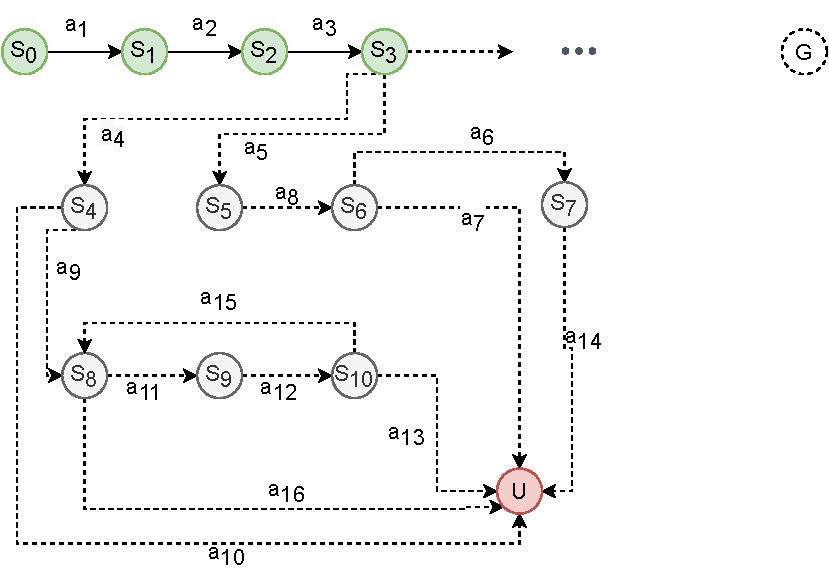
\includegraphics[width=0.8\columnwidth]{img/undesirable.pdf}}
	\caption{An application domain where a user executes the actions $a_1, a_2, a_3 $ to transform initial state $S_0$ to a goal state $G$. An undesirable state $U$ may develop from state $S_{3}$ after $a_3$ has been executed, following the plans ($\Pi_U$) indicated by the dotted paths towards $U$.}
\label{fig:cybersecproblem}
\end{figure}

\subsection{The Intervention Problem: Recognizing Undesirable Consequences}
Given a domain $\mathcal{D}$ and a planning problem $P$, an automated planner generates the planning task $\Pi=\langle \mathcal{F}, \mathcal{A}, I, G\rangle$, where $\mathcal{F}$ is a finite set of grounded propositions, $\mathcal{A}$ is the finite set of grounded actions instantiated from the operator schemata $Op$, $I$ is the grounded propositions specifying the initial state and $G$ is the grounded goal specification. Objects in $\mathcal{O}$ are used to ground $\mathcal{F}$, $\mathcal{A}$, $I$ and $G$. Grounding replaces the variable terms in the parameter lists of the propositions, action schema, goal specifications with constant/non-constant objects. 

We defined a domain model for the cyber-security domain using PDDL (Planning Domain Definition Language) a generalization of STRIPS, shown in Figure \ref{fig:cybersecdomain}. In total this domain model has 45 actions, 47 types, 70 constants and 55 predicates.
This STRIPS domain model captures the home computer user cyber-security scenarios simulated in the Psychorithm sandbox environment described in Chapter~\ref{chap:ch3}.

\begin{figure}[pbt]
\noindent\fbox{
 \parbox{\textwidth}{\raggedright: 
{\small
\texttt{(define (domain attackgraph-typed)}\\
\texttt{\hspace*{35pt}(:requirements :strips :adl :equality :typing \hspace*{35pt} :disjunctive-preconditions)}\\
        \hspace*{35pt}\texttt{(:types unknown software misc - object)\\
       \hspace*{35pt} \texttt{account certificate email-ID file key site user attacker vulnerability-type password direct-message device database parameter permission process username response request - misc}\\
\hspace*{35pt} \texttt{browser editor webmailer plug-in site-creating-software server-connecting-software server anti-virus OS desktop-app server-app malicious-software - software}\\
\hspace*{35pt} \texttt{phishing-site server-site normal-site - site}\\
\hspace*{35pt} \texttt{phishing-site-email phishing-site-twitter - phishing-site}\\
\hspace*{35pt} \texttt{attacker-remote attacker-local - attacker)}
        }\\ [15 pt]
\hspace*{35pt}\texttt{(:constants \\ 
\hspace*{35pt}user1-email-account user1-twitter-account - account \\
\hspace*{35pt}pc-doctor security-shield - anti-virus \\
\hspace*{35pt}browser-firefox - browser \\        \hspace*{35pt}phishing-direct-message - direct-message \\
\hspace*{35pt}email-with-malicious-attachment - email-ID\\
\hspace*{35pt}squirrelmail - webmailer\\
\hspace*{35pt}user1-twitter-password - password $\ldots$ )\\[15 pt]
}
\hspace*{35pt}\texttt{(:predicates \\
\hspace*{35pt}(information-available ?aUser - User ?anAccount - account) \\
\hspace*{35pt}(user-has-email-account ?anAccount - account)\\
\hspace*{35pt}(direct-message-received ?dmsg - direct-message)\\
\hspace*{35pt}(anti-virus-software-selected ?av - anti-virus) \\
\hspace*{35pt}(information-leakage ?anAccount - account $\ldots$ )\\[15pt]
}

\hspace*{35pt}(\texttt{:action user-visit-antivirus-download-site}\\
\hspace*{35pt}\texttt{:parameters (?U - user ?aBrowser - browser ?aSite - site \\\hspace*{35pt} ?av - anti-virus)}\\
\hspace*{35pt}\texttt{:precondition ( and (logged-onto-system ?U) \\\hspace*{35pt} (use-software ?aBrowser) (running ?aBrowser) \\\hspace*{35pt} (= ?aSite antivirus-software-download-site) \\\hspace*{35pt} (not (installed ?av))  (not (running ?av)) )}\\
\hspace*{35pt}\texttt{:effect (and (user-visits-site ?U ?aSite))}
)\\[15pt]

\hspace*{35pt}\texttt{(:action user-opens-attachment-through-webmail}\\
\hspace*{35pt}\texttt{:parameters (?U - user ?aBrowser - browser ?WM - webmailer \\\hspace*{35pt}?aSite - site  ?anAccount - account ?Msg - email-ID  ?F - file )}
\hspace*{35pt}\texttt{:precondition (and  (use-software ?aBrowser) (running ?aBrowser) \\\hspace*{35pt}(user-visits-site ?U ?aSite) (= ?aSite webmail-site)\\\hspace*{35pt}(user-has-email-account ?anAccount)\\\hspace*{35pt}(= ?anAccount user1-email-account) (msg-opened ?Msg)\\\hspace*{35pt}(mail-attachment ?Msg ?F) (logged-onto-system ?U))}\\
\hspace*{35pt}\texttt{:effect (opened ?F))} 
 )\\\hspace*{35pt}$\ldots\ldots$
}
}
}
\caption{The cyber-security PDDL domain model snippet}
\label{fig:cybersecdomain}
\end{figure}

\sloppy
\begin{definition}
An observation trace $O$ is a sequence of observed actions $O = \{o_1, o_2, ... ,o_n\}  \;where\; o_i\in \mathcal{A}\; and \; i=1,2, \dots ,n\; (n = $ length of observation trace) and states resulting from execution of actions $o_i\in O$ are known. 
\end{definition}

Traces may contain extraneous or missing actions.  An \emph{extraneous action} is an observation $o \in O$ such that the state resulting from executing $o$ is never added to the state (i.e., set of state variable predicates that are true) by any of the actions $a_i \in \pi_U$. A \emph{missing observation} with respect to $\pi_U$ occurs when the state resulting from executing $o$ is added to the global state by an of the actions $a_i \in \pi_U$, and $o \notin O$.

When we are looking for possible paths leading to an undesirable state, we search for a \textbf{undesirable plan} $\pi_U = \{a_1, \dots ,a_k\}$ of length $k$ that entails one or more undesirable states $U\subseteq \mathcal{F}$ and $a_i \in A$. There may be more than one undesirable plan, in which case we consider a set of undesirable plans $\Pi_U$. In the example in Figure \ref{fig:cybersecproblem}, the domain has only one undesirable state $U=\lbrace U_1\rbrace$.


\begin{definition}
An intervention problem $T = \langle \mathcal{D}, O, I, U \rangle$ consists of a planning domain $D$, a sequence of observed actions  $O \subseteq \mathcal{A}$, an initial state $I \subseteq \mathcal{F}$, a set of undesirable states $U\subseteq \mathcal{F}$.
\end{definition}
The solution to the intervention problem is a binary decision for each action in the observation trace, $o \in O;  o \rightarrow \lbrace Yes, No \rbrace$ indicating whether it was identified as a critical trigger action ($Yes$) or not ($No$).


\subsection{Identifying Critical Trigger Actions}
A \textbf{critical trigger action} $c_i$ is a  action at $o_i \in O, i\leq |O|$ that maximizes the metric function $V (c_i)$, which we define now.

We recognize two forms of candidate trigger actions in the observation trace: strong and weak. 
A strong trigger can actively contribute to causing the state (e.g., as an effect or by satisfying a required precondition) or allow another actor to cause it. 
A trigger may also weakly contribute to the causation of the undesirable state(s) and may not be worth intervening to prevent. 
Consequently, we add a layer to the intervention problem to support application specific ranking about which actions are most ``critical'', i.e., helpful in preventing the undesirable state(s). 
The key addition is an objective function that allows a tunable combination of metrics.

Our focus is on identifying the intervention point as early as  \textit{helpful} when a user may be triggering an undesirable state. 
The concept of helpful is similar to the value of alerts described in \cite{Wilkins2003} which recognized that it is important to be judicious in interrupting a user in scenarios where humans and machine agents interact with each other: ``don't ignore but don't annoy''. 
To this end, we start by defining a function composed of three  metrics to quantify the notion of helpfulness: \textbf{certainty}, \textbf{timeliness} and \textbf{desirability}. 
These metrics are calculated based on a set $\Pi_U$.


When producing the set of alternative undesirable plans $\Pi_U$, as representative of a set of possible trajectories toward an undesirable goal, it would be best to consider alternatives that are non-obvious and diverse from each other rather than just the optimal plan.  
This is especially important in long-running processes with complex traces or when a sub optimal plan contains a longer, but perhaps more easy to trigger, path to the undesirable state.

{\it Certainty} measures the likelihood of action $a$ occurring in $\Pi_U$.
\begin{equation}
\label{eq:certainty}
Certainty (a|\Pi_U)  = \frac{|\pi_U \in \Pi_U \textup{ in which}\; a\; \textup{occurs}|}{|\Pi_U|}
\end{equation}
Actions occurring frequently in $\Pi_U$ indicate the importance of that action toward causing $U$. For example, if an action $a$ occurs in all plans $\Pi_U$, the certainty metric will assign a high value to $a$, giving it a higher probability of being selected as a critical trigger compared to a less frequent action. 

{\it Timeliness} requires knowing what actions could yet be observed, which might effect the causation of the undesirable state. 
For this study, timeliness is measured by the maximum normalized steps remaining in $\Pi_U$ in which the action a occurs. 
Timeliness quantifies how soon an observation will trigger the undesirable state. 
Therefore, we compute the maximum in discrete time as opposed to the minimum because it indicate that an undesirable state is developing but not imminent and allows time to recover. 
Let $n$ be the remaining number of steps in $\pi_U \in \Pi_U$ after some action $a$. Then,
\begin{equation}
\label{eq:timeliness}
Timeliness (a|\Pi_U) = \max_{\pi_U \in \Pi_U}\left(\frac{
	\max\left( n \right)\
	}{\; |\pi_U|}\right) 
\end{equation}

{\it Desirability} measures the effect of an action on user's goals, which is ignored in the other two metrics. 
In the Intervention by Undesirable Consequence Recognition problem the intervening agent is only aware of the undesirable state the user wants to avoid.
Although the user's goal is hidden to the intervening agent, the intervention decision must also consider how the candidate trigger actions contribute toward the user's goal to allow some freedom for the user.
In Chapter~\ref{chap:ch3}, we showed that in the cyber-security domain, most actions users execute to accomplish a goal are harmless actions while only a few of them put the user at risk.
We capture this property with the Desirability metric and separate common harmless actions (e.g., user opening web browser) from avoidable ones and connects the observations to knowledge of the user's goals.
If an action appears often in the candidate trigger actions then that action is a common, harmless action and more desirable.
In contrast, actions that appear less often in the candidate trigger actions are comparatively more undesirable.
The intervening agent must consider the undesirable actions with higher priority.
Consequently we downgrade the contribution of the desirable actions to criticality by defining Desirability as a negative metric.
\begin{equation}
\label{eq:desirability}
Desirability (a|\Pi_U) = - \left( \frac{|\textup{appearance of}\; a\; \textup{ in } \Pi_U|}{\sum_{i=1}^{|\Pi_U|}\left | \pi_i \right |} \right)
\end{equation}
Together, these metrics define the function $V(a)$ for candidate trigger action $a$ for a weighting provided by $\alpha$, where $\alpha$ $=\lbrack\alpha_1, \ldots, \alpha_m \rbrack$, $\alpha_i$ is in the range $\lbrack0,1\rbrack$, $m$ is the number of objectives and $\sum_{1}^{m}\alpha_i = 1$:
\begin{equation}
\label{eq:function}
V(a) = (\alpha_1 \times Certainty (a|\Pi_U)) + (\alpha_2 \times Timeliness (a|\Pi_U)) + (\alpha_3 \times Desirability (a|\Pi_U))
\end{equation}

Table \ref{tab:metrics}, shows how the critical trigger action is identified using the proposed objective function for the example in Figure \ref{fig:cybersecproblem} given the observation sequence of actions $O=\{a_1, a_2, a_3\}$. 
In state $S_{3}$, assuming equal weighting of metrics, the algorithm identifies $a_{12}$ to be the action that maximizes the objective function, and returns it as a possible point of intervention. 
Table \ref{tab:metrics} also shows how this decision is affected by the choice of $\alpha$. If only certainty metric is used ($\alpha=\lbrack1,0,0\rbrack$) action $f$ gets selected as the intervention point. 
Using only timeliness metric ($\alpha=\lbrack0,1,0\rbrack$) yields three possible intervention points: $a_{12}$, $a_5$ and $a_4$. 
Finally, using only desirability yields four possible intervention points: $a_{10}$, $a_6$, $a_7$ and $a_{14}$.

\begin{table}[tpb]
	\centering
		\caption{Certainty (C), timeliness (T), desirability (D) computations for each candidate trigger action for the example in Figure \ref{fig:cybersecproblem}. $V(a)$ is the value returned by the critical trigger multi-objective function assuming equal weighting ($\alpha=\lbrack0.33,0.33,0.33\rbrack$), only C ($\alpha=\lbrack1,0,0\rbrack$), only T ($\alpha=\lbrack0,1,0\rbrack$) and only D ($\alpha=\lbrack0,0,1\rbrack$) for each candidate trigger action.}
\label{tab:metrics}
	\resizebox{\textwidth}{!}{
		\begin{tabular}{|c|l|l|l|c|c|c|c|}
			\hline
			\multirow{2}{*}{} & \multicolumn{1}{c|}{\multirow{2}{*}{C}} & \multicolumn{1}{c|}{\multirow{2}{*}{T}} & \multicolumn{1}{c|}{\multirow{2}{*}{D}} & \multicolumn{1}{l|}{$\alpha$ = {[}0.33,0.33,0.33{]}} & \multicolumn{1}{l|}{$\alpha$ = {[}1,0,0{]}} & \multicolumn{1}{l|}{$\alpha$ = {[}0,1,0{]}} & \multicolumn{1}{l|}{$\alpha$ = {[}0,0,1{]}} \\ \cline{5-8} 
			& \multicolumn{1}{c|}{} & \multicolumn{1}{c|}{} & \multicolumn{1}{c|}{} & $V(a)$ &$V(a)$ & $V(a)$ & $V(a)$  \\ \hline
			$a_5$ & 2/10=0.2 & max(3/3,4/4)=1.0 & -2/39=0.05 & 0.38 & 0.2 & \textbf{1.0} & -0.05 \\
			$a_4$  & 4/10=0.4 & max(2/2,3/3,5/5,6/6)=1.0 & -4/39=0.1 & 0.43 & 0.4 & \textbf{1.0} & -0.1 \\
			$a_{11}$  & 4/10=0.4 & max(3/5,4/6,3/5,4/6)=0.6 & -4/39=0.1 & 0.30  & 0.4 & 0.6 & -0.1 \\
			$a_{12}$  & 6/10=0.6  & max(2/5,3/6,2/2,3/3,5/5,6/6)=1.0  & -6/39=0.15 & \textbf{0.48} & \textbf{0.6}  & \textbf{1.0} & -0.15  \\
			$a_8$ & 2/10=0.2 & max(2/3,3/4)=0.75  & -2/39=0.05 & 0.30 & 
			0.2  & 0.75 & -0.05   \\
			$a_{10}$ & 1/10=0.1   & max(1/2)=0.5   & -1/39=0.03 & 0.19   & 0.1  & 0.5  & \textbf{-0.03}   \\
			$a_9$ & 3/10=0.3   & max(2/3,4/5,5/6)=0.83   & -3/39=0.08 & 0.35   & 0.3  & 0.83 & -0.08   \\
			$a_{15}$ & 4/10=0.4   & max(2/6,2/3,4/5,5/6)=0.83  & -6/39=0.15 & 0.36   & 0.4  & 0.83 & -0.15   \\
			$a_{13}$ & 3/10=0.3   & max(1/5,1/2,1/5)=0.5    & -3/39=0.08 & 0.24   & 0.3  & 0.5  & -0.08   \\
			$a_6$ & 1/10=0.1   & max(2/4)=0.5   & -1/39=0.03 & 0.19   & 0.1  & 0.5  & \textbf{-0.03}   \\
			$a_7$ & 1/10=0.1   & max(1/3)=0.33  & -1/39=0.03 & 0.13   & 0.1  & 0.33 & \textbf{-0.03}   \\
			$a_{16}$ & 4/10=0.4   & max(1/3,1/6,1/3,1/6)=0.33  & -4/39=0.1  & 0.21   & 0.4  & 0.33 & -0.1 \\
			$a_{14}$ & 1/10=0.1   & max(1/4)=0.25  & -1/39=0.03 & 0.11   & 0.1  & 0.25 & \textbf{-0.03}  \\ \hline
		\end{tabular}
	}%
\end{table}

Intervention is different from the typical plan recognition problem because the intervening agent assumes that the user pursues some desirable goal but wants to also avoid any undesirable state. 
Furthermore, the intervening agent has no knowledge about the user's desirable goal and knows only the set of undesirable states the user should avoid. 
Our model views the user's attempt to achieve a desirable goal as a planning process. 
Plan recognition approaches that use plan library representation do not apply for the Intervention problem because they are focused on matching observed actions to prior plans to determine what goals the user is trying to achieve.
The problems with that are: (1) the observations may contain extraneous actions and (2) the plans that lead to the undesirable states may not encompass the user's goal (the user does not want to trigger the vulnerability, but rather to do something useful with his computer).
Therefore, the objective is to identify intervention points based on their potential to cause the undesirable state, while making sure that the actions are identified in an \textit{opportune time}.

 
Our intervention model borrows ideas from the generative plan recognition approaches and analyses the Planning Graph and operates incrementally.
This is similar to prior work by Sun et al. \citeyear{sun2007recognizing} and Hong \citeyear{hong2001goal}. 
Following work by Geib and Goldman \citeyear{GeibGoldman09}, we adopt a model focused on execution: what could be done next. 
In contrast to the works of Ramirez and Geffner \citeyear{ramirez2009plan,ramirez2010probabilistic} that assumed a fully observable state space, our approach takes into consideration the inherent unreliable nature of observations (missing and irrelevant actions) towards identifying critical trigger actions. 
Our solution employs PDDL and the Mosaic planner \cite{roberts2014} to sample possible plans from the current state. 
For each observation, the algorithm outputs whether or not it is a critical trigger action. 

\subsection{Undesirable State Recognition Algorithm}
Figure~\ref{fig:components} shows the seven-step decision cycle of the algorithm. As defined in the problem statement, the process takes as input: a PDDL domain, an initial state, a set of undesirable states and the objective function weights. 

\textbf{Step 1:} We assume the full observation trace is known in advance, with actions made available one at a time to identify the intervention point. However, the algorithm does not utilize information that can be gleaned from the full trace to yield the decision. Input to the algorithm in this step can also be replaced with application specific sensors.  

\textbf{Step 2:} For each possible undesirable state $U$, generate PDDL problem instances. In the first cycle, the initial state is from the input; in subsequent cycles, the state is updated in step 7. To extract applicable states for the next cycle, we chose to search forward the planning graph starting from initial state. This is because the unobservable actions require us to update state during search to accommodate those changes that are presupposed by the actions being able to execute. 

\textbf{Step 3:}
We opted to apply a diverse planner.  
A recent study examined the impact of diversity metrics in classical planning  \cite{roberts2014}, and a contribution from that work, the Mosaic planner, produces a set of diverse plans in a single run. 
A key finding by the authors of Mosaic was that existing diverse planners frequently produce plan sets containing actions not leading to the goal, which increased diversity but lacked justification for many applications. 
Mosiac returns $\Pi_U$ for $U$. 

Mosaic is built on top of the LAMA planner \cite{richterWestphal10.jair.LAMA}  with some patches applied to its parser from the current Fast Downward repository\footnote{See \smallurl{http://www.fast-downward.org/}}. It included three extensions to improve the plan set and produce diverse plans faster: the use of a tabu mechanism to guide search away from already known solutions, the use of multiple queues to increase the diversity of solutions explored, and the use of parsimony to bias the search toward goal-oriented solutions. From the family of variants, iterated Tabu A* (ITA) and Multi-queue A* (MQA), we use MQA-TS to compute up to 10 possible plans, based both on the recommendation of the authors and because it showed the most promise in prior work. 

\textbf{Step 4:} Extract unique actions in $\Pi_U$ as candidate trigger actions. Actions include the action name and the instantiated parameter values.

\textbf{Step 5:} Compute Certainty, Timeliness and Desirability for each candidate trigger action by iterating over the plans in $\Pi_U$, as defined in Function \ref{eq:function}. 

\textbf{Step 6:} Rank candidate actions by $V$. Flag the highest ranked actions as critical triggers corresponding to the current observation. Step 6 also evaluates the accuracy of the identified critical trigger by comparing against the observation. 
We use a ground-truth \textbf{u}ndesirable \textbf{p}lan (called UP) that achieves the undesirable state and assume that all actions in the ground-truth undesirable plan are critical triggers. 
If the algorithm returns the current observation as the critical trigger, then the decision is correct if the current observation is an action in the ground-truth undesirable plan (i.e., true-positive). 
Alternatively, if the current observation is not the critical trigger and it was also missing in the ground-truth undesirable plan (i.e., observation was an extraneous action and a true-negative), then that decision is also labeled as correct. 
All other cases are incorrect.

\textbf{Step 7:} The cycle begins over by merging the effects of the observed action as defined in the PDDL domain with the current state. 
Because we allow for partial observability, the observed action may appear to be inapplicable because actions that satisfied its preconditions were not observed and so captured by the current state. 
Our approach addresses this inconsistency in state by finding a plan that modifies current state to the state after adding the effects of the observed action. 
Then, each action in that plan are executed (i.e., adding add effects, removing delete effects) to update the current state.

\begin{figure}[t]
\centering{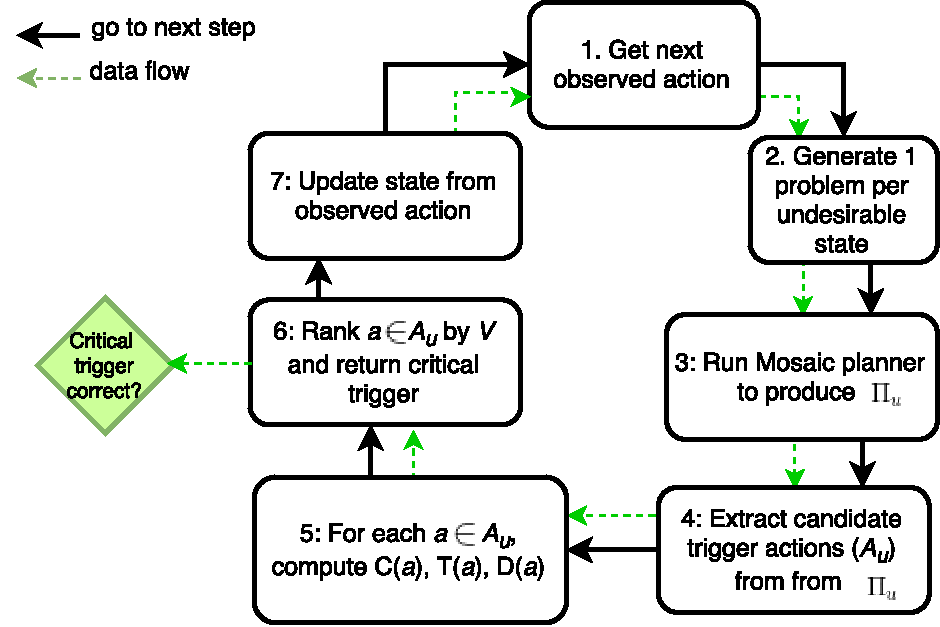
\includegraphics[width=0.7\textwidth]{img/algorithm.pdf}}
\caption{Seven-step process for determining whether an observed action is a critical trigger action.}
\label{fig:components}
\end{figure}

\section{Evaluating the Undesirable Consequence Recognition}
We examine which factors impact the performance of detecting critical trigger actions using our metric function $V$. The \emph{independent variables} of the study are summarized in Table~\ref{tab:exp}, and include the weights for V, the problems, the percentage of extraneous actions, and the percentage of actions ``removed'' to emulated partial observability.

Objective weights vary between a single metric, pairs of metrics and all three metrics with equal weights. We decided on these objective weight settings in order to identify which metrics (or their combinations) are sensitive to partial observability and extraneous actions separately. 


We begin with results from a user study on cyber-security that motivated our work. This domain will be referred to as the \texttt{PAG} in our evaluation. For traces from the user study, we examine the impact of the objective weights (OW) used for in the objective function. Noisy sensing can lead to extraneous actions or missed observations, which complicates intervention. So we generalize these results to a set of benchmark domains from \cite{ramirez2009plan}, where greater experimental control allows us to evaluate the impact of extraneous actions (EA) and partial observability (PO). Thus, we expect some degradation in performance as the noise increases and observability decreases; the question is by how much? 

\begin{table}[tpb]
\caption{Independent variables for evaluating impact of algorithm parameters and sensitivity to noisy data}
\label{tab:exp}
\begin{tabular}{|l|l|}
\hline
Variable                   & Settings                                           \\ \hline
\begin{tabular}[c]{@{}l@{}}Objective Weights (OW)\\ (C,T,D)\end{tabular} &
  \begin{tabular}[c]{@{}l@{}}(1,0,0), (0,1,0), (0,0,1), (0.33,0.33,0.33), (0.5,0.5,0), \\ (0.5,0,0.5), (0,0.5,0.5)\end{tabular} \\ \hline
Planning Domains (PD)       & PAG, blocks-words, navigator, ipc-grid+, logistics \\ \hline
Partial observability (PO) & 25\%, 50\%, 75\%, 100\%                            \\ \hline
Extraneous Actions (EA)    & 0\%, 50\%, 75\%, 100\%                             \\ \hline
\end{tabular}
\end{table}


The \emph{dependent variables} of the study include accuracy and computational overhead as measured in CPU time. For the cybersecurity domain, accuracy is defined as the percent true-positives only. For the benchmarks, we report accuracy in terms of percent true-positives and true-negatives. Computation time is included because ultimately we envision this being one component of a user supporting agent, which will require fast response. CPU time includes the time required to process each observation (one cycle of the process depicted in Figure~\ref{fig:components}) within a trial; this includes both generating the alternate plans and ranking the actions. 

For each undesirable state, we use a plan generated by an automated planner as the ground-truth undesirable plan. 
This is a fair assumption because the trace generation algorithm produces traces leading to the undesirable state (with varying levels of noise and observability). 
We measure accuracy with two evaluation metrics:
\begin{itemize}
\item Success rate in ignoring extraneous actions (Ignored EA)
\item Success rate in flagging undesirable actions that appear in the ground truth undesirable plan (Flagged UP)
\end{itemize}

Ignored EA for an observation trace is computed as the count of instances where the observation was an extraneous action and it was not flagged as a critical trigger (count EA). It is given by the equation:
\begin{equation}
\textup{Ignored EA}\%= \frac{\textup{count EA}}{\textup{number of extraneous actions in trace}}\times 100
\end{equation}
Flagged UP for an observation trace is computed as the count of instances where the observation was an action from UP and the function V actually selected it as the critical trigger action. It is given by the equation:
\begin{equation}
\textup{Flagged UP}\%= \frac{\textup{count UP}}{\textup{number of UP actions in trace}}\times 100
\end{equation}

\subsection{Cyber-security Domain (PAG)}
In Chapter~\ref{chap:ch3}, we discussed the findings of an human subject experiment where users performed routine computer tasks in a sandboxed simulation environment.
The objective of this study was to determine how non-expert users behave when presented with questionable computer security situations and to compare their actual observed behavior to their self-reports obtained via pre- and post-hoc surveys. 
Participants were presented with a desktop which includes common applications such as emailing, Web-browsing, social networking etc. 
They were also provided with written instructions on how to perform normal home computer user activities such as reading/sending email, installing software etc. While the normal computer activities were being performed, different events were simulated, without the subject's knowledge that can trigger threats and vulnerabilities of interest. 
These events included enticing user to disclose sensitive information (login names, passwords) to phishing sites over email and social media communications, responding to pop-ups asking the user to download a software, and reacting to malicious activities detected in the computer by an anti-virus program. 
Sixty-three human subjects participated in the study; their actions were collected into observation traces and will be used in the evaluation of our undesirable consequences recognition algorithm.


We constructed a PDDL domain for the Personalized Attack Graph (\texttt{PAG}) to investigate what actions subjects might take amid the aforementioned threat scenarios.  We considered four undesirable states for this domain, resulting in four problem definitions. Figure~\ref{fig:trace} shows an actual observation trace indicating how the subject's observed actions (x axis) contributed to triggering the four undesirable states (the plans to do so are displayed as a sequence in each color). The y-axis shows how many steps in each undesirable plan (UP) have yet to be executed. When the dots remain horizontal, the actions are not in the undesirable plan; they are extraneous. For this trace, although the subject came close to triggering all four, only one actually happened (red color line - virus scan vulnerability). 

\begin{figure}[tpb]
 \centerline{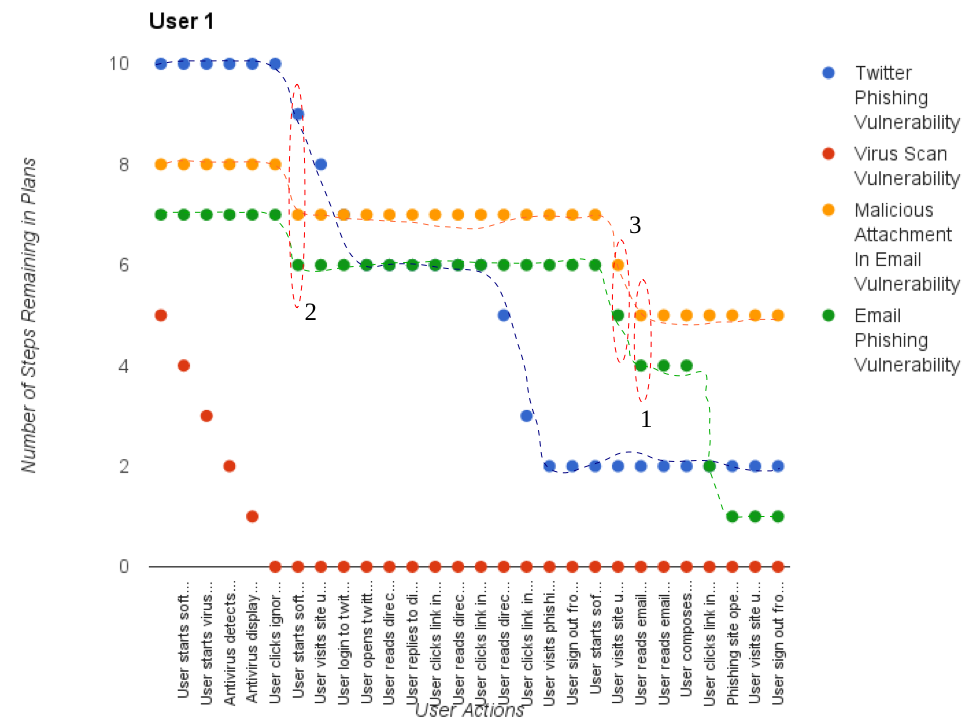
\includegraphics[width=\columnwidth, keepaspectratio=true]{img/user-study.png}}
 \caption{Observation trace from a human subject annotated with relation to undesirable plans (colored connected dots) and candidate trigger actions (in dotted ovals)}
 \label{fig:trace}
\end{figure}

We expected accuracy to be low because user logs offer unique challenges to the algorithm. Human users do not typically perform tasks in an ordered sequence. For example, some logs indicated that the subject was performing the same task repetitively, users had skipped a task to come back to it after an interval and more interestingly, some users were actively trying to trigger the vulnerabilities. These scenarios make it difficult to model a consistent state in a planning environment and affect candidate trigger actions being selected for the critical trigger ranking algorithm. To assess algorithm performance in a more controlled environment, we turned to benchmarks.


\subsubsection{PAG Results}
Since activity logs captured during the experiment could not be properly controlled for extraneous and missing actions, we limit the assessment to accuracy and the effect of the metric weightings on Flagged UP accuracy and CPU usage.

The subjects were only provided with instructions to perform normal computer tasks. No restrictions were imposed on how they should interact with desktop environment (e.g., undo/redo tasks, exploring application features). Therefore, subject's goals while performing the tasks were unknown. Logs generated by two subjects were discarded because they did not complete the experiment. Considering 61 traces used in this evaluation, mean trace length was 39 (SD=21.13). The longest trace contained 120 observations, while the shortest was 10. 


Mean Flagged UP accuracy was 59.53\% (SD=30.79) across all metric weight assignment classes, but the weights exerted a significant influence on accuracy (\textit{F}=40866, \textit{p}$\ll$0). 
The highest accuracy (mean=95.59\%,SD=2.13) occurred for two configurations of metric weight assignments: one that equally weighted Certainty, Desirability and Timeliness metrics as well as the one that equally weighted Certainty and Timeliness, ignoring the Desirability metric. 
We find that, in the cyber-security domain, the Undesirable Consequence Recognition algorithm relies on the Certainty and Timeliness metrics the most.
Mean CPU time per cycle of the algorithm was 1.7 seconds (SD=0.45), suggesting that this algorithm could easily be integrated into an agent that mitigates cyber-security issues.


\subsection{Benchmark Domains}
To generalize the results, we examine four domains from \cite{ramirez2009plan}. 
\sloppy
{\tt Block-Words} constructs one of 20 English words using 8 distinct letters. {\tt Grid-Navigation} forms paths through a connected graph to specific locations (goals). {\tt IPC-grid+} is a grid navigation with keys added at a restricted set of locations. {\tt Logistics} moves packages between locations. To keep the scale similar to the user study, we randomly selected four problems from each domain distribution.

\subsubsection{Trace Generation}
We choose four undesirable states for each benchmark domain.
To construct problem factors, partial observability and extraneous actions, we construct four planning problems with the undesirable states set as the goals. 
For each problem, we generate noisy traces by incrementally building the plan starting from the initial state and interleaving it with actions from a set of pre-computed extraneous actions when the current state meets the preconditions of the extraneous action. 
Thus, the trace generation algorithm consists of two stages (1) computing the set of extraneous actions (EA) and (2) interleaving these extraneous actions in to the trace. 
To construct partial observability (PO), actions from the original ground truth 
undesirable plan are randomly removed from the interleaved trace.

We use the Metric-FF planner \cite{hoffman2003ff} to generate extraneous actions because the planner's implementation offers configuration options to extract the relaxed planning graph and add/delete effects of actions. 
The challenge in generating extraneous actions is to ensure that they (1) do not introduce new facts that interfere with the progression of the ground-truth undesirable plan  or (2) does not delete the progress already made by the ground truth undesirable plan. 

First, we incrementally build the set of extraneous actions starting from selecting actions that can be executed immediately after the goal state has been reached. 
By adding new actions, object types, and predicates to the domain model, the size of the resulting extraneous action set can be increased to handle longer plans and create lengthy traces. 
The advantage of forward-expanding the set of extraneous actions starting at the goal state is that at this stage, the only condition we need to check is whether or not the chosen action deletes the goal state or not.
We add the actions that do not delete the goal state predicates as extraneous actions. 
It is also possible to select extraneous actions from the applicable actions in the current level of the Relaxed Planning Graph.
However, this does not guarantee that these actions will not violate conditions (1) and (2) later in the plan. 
In certain occasions selecting extraneous actions this way could lead to traces where the same action is being done and undone repeatedly without making progress through the plan, which is unrealistic and not rational behavior.

 
We designed a trace generation algorithm that overcomes the aforementioned problems and builds the ground-truth undesirable plan incrementally from the initial state, while interleaving it with extraneous actions.
Algorithm \ref{alg:extraneous} describes the process to compute the extraneous action pool for each problem in a domain.
\begin{algorithm}
    \caption{Extraneous Action Generation Algorithm}
    \label{alg:extraneous}
    \begin{algorithmic}[1]
        \Procedure{extraneouspool}{$domain$,$undesirableState,init$}
        	\State $current\gets UP, EX_{goal}\gets \emptyset, state \gets \emptyset$
        	\State $UP\gets Planner(domain,undesirableState,init)$
        	\State $state \gets init$
        	\ForAll{$a \in current$}
        		\If{$Pre(a)\in state $} 
        		\State $state\gets state\setminus Del(a)\cup Add(a)$
        		\EndIf
        	\EndFor
        	\State $S_{g}\gets state$
        	\State $RPG \gets RelaxedPlanningGraph(domain,undesirableState,init)$
        	\ForAll {$action \in RPG$}
				\If{$(action \notin UP) \And (Pre(action) \in S_{g}) \And (state \setminus Del(action) \cup Add(action) \cap S_{g} = \emptyset)$} 
				\State $EX_{g} \gets action$
				\EndIf        	        	
           	\EndFor
            \State \textbf{return} $EX_{g}$
        \EndProcedure
    \end{algorithmic}
\end{algorithm}
We begin by computing the ground-truth undesirable plan $UP$ using a planner. 
Then for the actions in $UP$ we modify the initial state by incorporating the effects of each action. 
The end of this loop translates the $state$ to the goal state for the problem. 
Then we generate the Relaxed Planning Graph for the planning problem with the goal equal to the undesirable state.
We select actions from the Relaxed Planning Graph such that the actions that are not already in $UP$ and the selected action is applicable in the goal state and post-conditions of the selected action do not remove any goal predicates. 
These actions form the extraneous action pool $EX_{g}$.
The set $EX_{g}$ needs to be extended because we evaluate the Undesirable Consequence Recognition algorithm by varying the percentage of extraneous actions in the observation trace.
This is done by modifying $S_{g}$ with effects of a selected action from $EX_{g}$, and repeating steps 4 through 5. 
The intuition is that once an extraneous action is executed at some state, the resulting state may enable additional extraneous actions. 
Repeat execution of this process generates a tree structure of extraneous actions with an action from $EX_{g}$ as root. 

For an observation trace, we define the metric percent extraneous actions (EA) as follows:
\begin{equation}
\textup{percent extraneous actions (EA)} = \frac{\textup{number of extraneous actions in trace}} {\textup{number of actions in plan}}
\end{equation} 
This metric is used as a proxy for signal-to-noise ratio $[$0\%, 50\%, 75\%, 100\%$]$. 
Algorithm \ref{alg:noisytrace} describes our trace generation process. 
Starting from the initial state, actions in the undesirable plan are added to the observation trace sequentially, including extraneous actions as appropriate. 
This produces a final plan. 
Partial observability (PO) is computed by randomly removing actions from the final plan such that, PO\% (number of original actions in trace after removal / number of original actions in trace before removal) is one of $[$25\%, 50\%, 75\%, 100\%$]$. 

\begin{algorithm}
    \caption{Noisy Observation Trace Generation Algorithm}
    \label{alg:noisytrace}
    \begin{algorithmic}[1] % The number tells where the line numbering should start
        \Procedure{noisytrace}{$domain$,$problem,init$}
        	\State $current\gets UP, ea\gets 0, trace\gets \emptyset, state \gets init$
        	\State $UP\gets Planner(domain,problem,state)$
        	\ForAll{$a \in current$}
        		\If{$Pre(a)\in state $} 
        		\State $trace \gets trace \cup a$
        		\State $state\gets state\setminus Del(a)\cup Add(a)$
        		\EndIf
        		\State $UP\gets Planner(domain,problem,state)$
        		\State $current\gets UP$
        		\If {$ea<required EA\%$}
        		\State randomly select $action$ from $EX_{goal}$ if Pre($action$) $\in state$
        		\State $trace \gets trace \cup action$
        		\State update $ea, state, current$
        		\EndIf
        	\EndFor
        	\State Fix PO\% in $trace$ by removing actions
            \State \textbf{return} $trace$
        \EndProcedure
    \end{algorithmic}
\end{algorithm}





   \begin{table}[tpb]
     \centering
   \begin{small}
   	\caption{Mean Ignored EA\%  (and standard deviation) for benchmark domains for levels of EA\% in observation trace and objective weight assignment classes. The left three columns combine mean Ignored EA\% for OW assignments across all values of $\alpha$ and breaks mean Ignored EA\% down by EA\% in trace. The right OW columns breaks down mean Ignored EA\% by specific $\alpha$ value for all levels of EA\% in observation trace.}
	\label{tab:ignoredeaforlevels}
   \resizebox{\columnwidth}{!}{
	\begin{tabular}{|c|ccc|ccccccc|}
		\hline
	    & \multicolumn{10}{c|}{Mean Ignored EA\%} \\ \cline{2-11}
		\multirow{3}{*}{Domain}  & \multicolumn{3}{c|}{EA\% in trace} & \multicolumn{7}{c|}{OW Assignments  (C,T,D)} \\ \cline{2-11} 
		& 50\% & 75\% & 100\%
%		& (0,0,1) & (0,.5,.5) & (0,1,0) & (.3,.3,.3) & (.5,0,.5) & (.5,.5,0) & (1,0,0) \\ \hline
		& (0,0,1) & (0,0.5,0.5) & (0,1,0) & (0.3,0.3,0.3) & (0.5,0,0.5) & (0.5,0.5,0) & (1,0,0) \\ \hline
		\texttt{blo} & \begin{tabular}[c]{@{}c@{}}95.2 \\ (8.0)\end{tabular} & \begin{tabular}[c]{@{}c@{}}97.6\\ (3.6)\end{tabular} & \begin{tabular}[c]{@{}c@{}}97.3\\ (3.2)\end{tabular} & \begin{tabular}[c]{@{}c@{}}99.0\\ (1.6)\end{tabular} & \begin{tabular}[c]{@{}c@{}}94.7\\ (6.7)\end{tabular} & \begin{tabular}[c]{@{}c@{}}95.2\\ (6.2)\end{tabular} & \begin{tabular}[c]{@{}c@{}}95.4\\ (7.0)\end{tabular} & \begin{tabular}[c]{@{}c@{}}98.6\\ (1.7)\end{tabular} & \begin{tabular}[c]{@{}c@{}}95.4\\ (7.0)\end{tabular} & \begin{tabular}[c]{@{}c@{}}98.6\\ (1.7)\end{tabular} \\ \hline
		\texttt{ipc} & \begin{tabular}[c]{@{}c@{}}86.4\\ (14.4)\end{tabular} & \begin{tabular}[c]{@{}c@{}}89.9\\ (11.6)\end{tabular} & \begin{tabular}[c]{@{}c@{}}89.9\\ (10.7)\end{tabular} & \begin{tabular}[c]{@{}c@{}}95.6\\ (3.7)\end{tabular} & \begin{tabular}[c]{@{}c@{}}83.2\\ (13.0)\end{tabular} & \begin{tabular}[c]{@{}c@{}}81.3\\ (12.9)\end{tabular} & \begin{tabular}[c]{@{}c@{}}83.9\\ (15.1)\end{tabular} & \begin{tabular}[c]{@{}c@{}}95.9\\ (3.4)\end{tabular} & \begin{tabular}[c]{@{}c@{}}85.1\\ (14.8)\end{tabular} & \begin{tabular}[c]{@{}c@{}}95.9\\ (3.4)\end{tabular} \\ \hline
		\texttt{log} & \begin{tabular}[c]{@{}c@{}}97.9 \\ (4.4)\end{tabular} & \begin{tabular}[c]{@{}c@{}}96.7\\ (5.7)\end{tabular} & \begin{tabular}[c]{@{}c@{}}96.1\\ (5.4)\end{tabular} & \begin{tabular}[c]{@{}c@{}}98.4\\ (2.8)\end{tabular} & \begin{tabular}[c]{@{}c@{}}94.4\\ (7.2)\end{tabular} & \begin{tabular}[c]{@{}c@{}}96.1\\ (3.6)\end{tabular} & \begin{tabular}[c]{@{}c@{}}96.2\\ (6.9)\end{tabular} & \begin{tabular}[c]{@{}c@{}}98.6\\ (2.6)\end{tabular} & \begin{tabular}[c]{@{}c@{}}96.2\\ (6.9)\end{tabular} & \begin{tabular}[c]{@{}c@{}}98.5\\ (2.6)\end{tabular} \\ \hline
		\texttt{nav} & 100 (0) & 100 (0) & 100 (0) & 100 (0) & 100 (0) & 100 (0) & 100 (0) & 100 (0) & 100 (0) & 100 (0) \\ \hline
	\end{tabular}
	}%	
   \end{small}
\end{table}


\begin{table}[tpb]
	\centering
\begin{small}
\caption{Mean Flagged UP\%  (and standard deviation) for benchmark domains for levels of PO\% in observation trace and objective weight assignment classes. The left four columns combine mean Flagged UP\% for OW assignments across all values of $\alpha$ and breaks mean Flagged UP\% down by PO\% in trace. The right OW columns breaks down mean Flagged UP\% by specific $\alpha$ value for all levels of PO\% in observation trace.}
	\label{tab:flaggedupforlevels}
\resizebox{\columnwidth}{!}{
	\begin{tabular}{|c|c c c c|c c c c c c c|}
		\hline
		& \multicolumn{11}{c|}{Mean Flagged UP\%} \\ \cline{2-12} 
		\multirow{3}{*}{Domain} & \multicolumn{4}{c|}{PO\% in trace} & \multicolumn{7}{c|}{OW Assignments (C,T,D)} \\ \cline{2-12} 
%		& 25\% & 50\% & 75\% & 100\% & (0,0,1) & (0,.5,.5) & (0,1,0) & (.3,.3,.3) & (.5,0,.5) & (.5,.5,0) & (1,0,0) \\ \cline{1-12} 
		& 25\% & 50\% & 75\% & 100\% & (0,0,1) & (0,0.5,0.5) & (0,1,0) & (0.3,0.3,0.3) & (0.5,0,0.5) & (0.5,0.5,0) & (1,0,0) \\ \cline{1-12} 
		
		\texttt{blo} & \begin{tabular}[c]{@{}c@{}}20.1\\ (21.2)\end{tabular} & \begin{tabular}[c]{@{}c@{}}23.6\\ (14.4)\end{tabular} & \begin{tabular}[c]{@{}c@{}}31.8\\ (19.3)\end{tabular} & \begin{tabular}[c]{@{}c@{}}40.2\\ (26.1)\end{tabular} & \begin{tabular}[c]{@{}c@{}}9.2\\ (7.6)\end{tabular} & \begin{tabular}[c]{@{}c@{}}24.8\\ (20.1)\end{tabular} & \begin{tabular}[c]{@{}c@{}}37.0\\ (17.5)\end{tabular} & \begin{tabular}[c]{@{}c@{}}46.5\\ (24.9)\end{tabular} & \begin{tabular}[c]{@{}c@{}}19.0\\ (7.6)\end{tabular} & \begin{tabular}[c]{@{}c@{}}46.8\\ (24.9)\end{tabular} & \begin{tabular}[c]{@{}c@{}}19.0\\ (7.6)\end{tabular} \\ \hline
		\texttt{ipc} & \begin{tabular}[c]{@{}c@{}}6.9\\ (18.8)\end{tabular} & \begin{tabular}[c]{@{}c@{}}25.6\\ (20.0)\end{tabular} & \begin{tabular}[c]{@{}c@{}}42.3\\ (32.0)\end{tabular} & \begin{tabular}[c]{@{}c@{}}50.8\\ (36.2)\end{tabular} & \begin{tabular}[c]{@{}c@{}}9.7\\ (5.2)\end{tabular} & \begin{tabular}[c]{@{}c@{}}46.5\\ (34.7)\end{tabular} & \begin{tabular}[c]{@{}c@{}}47.9\\ (35.0)\end{tabular} & \begin{tabular}[c]{@{}c@{}}47.5\\ (35.8)\end{tabular} & \begin{tabular}[c]{@{}c@{}}10.5\\ (4.9)\end{tabular} & \begin{tabular}[c]{@{}c@{}}47.1\\ (35.9)\end{tabular} & \begin{tabular}[c]{@{}c@{}}10.6\\ (4.9)\end{tabular} \\ \hline
		\texttt{log} & \begin{tabular}[c]{@{}c@{}}18.4\\ (27.4)\end{tabular} & \begin{tabular}[c]{@{}c@{}}16.4\\ (20.1)\end{tabular} & \begin{tabular}[c]{@{}c@{}}20.4\\ (19.5)\end{tabular} & \begin{tabular}[c]{@{}c@{}}31.5\\ (17.8)\end{tabular} & \begin{tabular}[c]{@{}c@{}}15.2\\ (10.6)\end{tabular} & \begin{tabular}[c]{@{}c@{}}20.9\\ (28.2)\end{tabular} & \begin{tabular}[c]{@{}c@{}}24.6\\ (25.4)\end{tabular} & \begin{tabular}[c]{@{}c@{}}27.2\\ (28.5)\end{tabular} & \begin{tabular}[c]{@{}c@{}}18.3\\ (10.1)\end{tabular} & \begin{tabular}[c]{@{}c@{}}27.2\\ (28.5)\end{tabular} & \begin{tabular}[c]{@{}c@{}}18.3\\ (10.9)\end{tabular} \\ \hline
		\texttt{nav} & \begin{tabular}[c]{@{}c@{}}14.8\\ (19.1)\end{tabular} & \begin{tabular}[c]{@{}c@{}}32.4\\ (22.6)\end{tabular} & \begin{tabular}[c]{@{}c@{}}45.2\\ (27.4)\end{tabular} & \begin{tabular}[c]{@{}c@{}}61.7\\ (39.8)\end{tabular} & \begin{tabular}[c]{@{}c@{}}14.1\\ (3.4)\end{tabular} & \begin{tabular}[c]{@{}c@{}}56.8\\ (33.7)\end{tabular} & \begin{tabular}[c]{@{}c@{}}56.8\\ (33.7)\end{tabular} & \begin{tabular}[c]{@{}c@{}}56.8\\ (33.7)\end{tabular} & \begin{tabular}[c]{@{}c@{}}14.1\\ (3.43)\end{tabular} & \begin{tabular}[c]{@{}c@{}}56.8\\ (33.7)\end{tabular} & \begin{tabular}[c]{@{}c@{}}14.1\\ (3.4)\end{tabular} \\ \hline
	\end{tabular}
	}%
\end{small}
\end{table}



\subsubsection{Benchmark Results}
We review the overall accuracy of our algorithm in benchmark domains by evaluating how well it ignores extraneous actions and flags undesirable actions in the ground truth plan.

\textbf{Ignoring Extraneous Actions}\\
When encountered with extraneous actions in the trace, the algorithm must be able to avoid flagging it as critical. We define mean Ignored EA\% percentage for a domain as: (sum of Ignored EA\% per trial / number of trials with EA\%$>$0). Table \ref{tab:ignoredeaforlevels} shows how mean Ignored EA\% varies with the noise level of the observation trace and objective weight assignments.

Results show that our algorithm consistently ignores extraneous actions for all benchmark domains. This high accuracy rate can be attributed to our process of selecting critical trigger actions. Since candidate trigger actions are extracted from a set of alternative plans leading to the same undesirable state, the likelihood of true extraneous actions to appear in the set of alternative plans is low. This reduces the likelihood of false-positives in the trace.


The OW combinations significantly influence Ignored EA\%  ($p<0.05$ for the \texttt{blo}, \texttt{ipc} and \texttt{log} domains). Post-hoc analysis using TukeyHSD at $\alpha=0.05$ shows that across domains, OW combinations that do not consider the timeliness metric better perform at ignoring extraneous actions than combinations that include timeliness. This is because timeliness metric is not sensitive to extraneous actions in the trace. As a result, the objective function can not sufficiently differentiate between extraneous actions and actions in ground truth plan, leading to false positives.Because timeliness metric captures progress yet to be made from current state to triggering the undesirable state in terms of remaining steps, in the presence of extraneous actions, which do not contribute to progress toward the undesirable state, the metric does not sufficiently demote the extraneous action in the candidate action set, leading to false-positives. 
In contrast, certainty and desirability metrics look for occurrences of an action in undesirable plans. As extraneous actions do not occur in undesirable plans, both metrics are capable of filtering extraneous actions from the candidate action pool by minimizing objective function value and preventing them from being selected as the critical trigger.


\textbf{Flagging Undesirable Actions}\\
Flagged UP\% captures how well the algorithm flags observations as critical triggers given that the observation appears in an undesirable plan treated as ground truth. We first look at Flagged UP\% in traces with 0\% noise and full observability (i.e., best-case scenario) to establish an upper bound to the metric.

Table \ref{tab:flagupupperbound} shows a very large range (Max-Min) for Flagged UP\%. This indicates that although the only variable for this sample is OW, Flagged UP\% is also sensitive to other external factors that have not been accounted for in our proposed objective function. The challenge lies in identifying these external factors and determining their relationship so that the objective function can be tuned to improve accuracy. This will be the main focus of our future work. 

Table \ref{tab:flaggedupforlevels} shows that Flagged UP\% also increases when observability increases in the trace. Factor analysis using one-way ANOVA for OW shows that this positive effect is significant ($p<0.05, df=6$) for all four benchmark domains. Interestingly, high Flagged UP\% was reported for OW combinations that consider timeliness: specifically for configurations, certainty-timeliness-desirability with equal weighting, certainty-timeliness with equal weighting and desirability-timeliness with equal weighting. Post-hoc analysis using TukeyHSD at $\alpha=0.05$ shows that this difference is significant. Thus, we conclude that the timeliness metric can improve the true-positive rate, yielding higher precision for the algorithm. The timeliness metric is sensitive to partial observability because it sufficiently captures distance to triggering an undesirable state, which is a consistent indicator of the progress is being made. Even with partial observability, the remaining steps of a plan change in such a way that it can be tracked and correctly reflected in the objective function. Accuracy of the certainty and desirability metrics lowers as partial observability increases because they consider occurrences of an action. 


\textbf{Computational Overhead}\\
For each benchmark domain, we calculated the average CPU time per cycle for problem factors (EA and PO). As shown in Table \ref{tab:cpu2}, we found differences due to observation trace factors; two-way ANOVA on EA and PO showed significant main effects and interaction effects ($p<$0.05) for \texttt{ipc}, \texttt{log} and \texttt{nav} domains.


\begin{table}[tpb]
  \centering
    \caption{Mean CPU time in seconds for problem factors for each domain. $\Delta$ is the difference between the max and min times for each domain.}
  \label{tab:cpu2}
    \resizebox{0.7\columnwidth}{!}{
  \begin{tabular}{|l|r|r|r|r|r|r|r|r|r|}
    \hline
    \multirow{2}{*}{Domain}
  &  \multicolumn{4}{c|}{EA\% in trace} & \multicolumn{4}{c|}{PO\% in trace} & \\ \cline{2-9}
 & 0\% & 50\% & 75\% & 100\% & 25\% & 50\% & 75\% & 100\% & $\Delta$ \\
    \hline
{\tt blo} & 2.3  & 2.2  & 2.2  & 2.2  & 2.2  & 2.2  & 2.3  & 2.2  & 1.4  \\
{\tt ipc} & 4.9  & 4.8  & 4.9  & 4.9  & 4.9  & 4.9  & 4.9  & 4.8  & 0.9  \\
{\tt log} & 1.7  & 1.7  & 1.6  & 1.7  & 1.7  & 1.7  & 1.7  & 1.7  & 0.5  \\
{\tt nav} & 1.3  & 1.3  & 1.3  & 1.3  & 1.3  & 1.3  & 1.3  & 1.3  & 0.5  \\
    \hline
  \end{tabular}
  	}%resize box
\end{table}

\begin{table}[tpb]
	\centering
\caption{Flagged UP\% for traces with 0\% EA and 100\% PO for \texttt{Block-words} (\texttt{bw}), \texttt{IPC-grid+} (\texttt{ipc}), \texttt{Logistics} (\texttt{log}), and \texttt{Grid-Navigation}   (\texttt{nav}) domains}
		\label{tab:flagupupperbound}
    \begin{small}
	\begin{tabular}{|l|c|c|c|c|}
		\hline
		\multirow{2}{*}{Domain} & \multicolumn{4}{c|}{Flagged UP\%} \\ \cline{2-5} 
		& Mean   & SD     & Min    & Max    \\ \hline
		\texttt{blo}                     & 37.12  & 24.83  & 6.12   & 77.78  \\ 
		\texttt{ipc}                     & 43.27  & 30.55  & 0.00   & 90.00  \\ 
		\texttt{log}                     & 31.77  & 17.27  & 12.82  & 66.67  \\ 
		\texttt{nav}                     & 61.68  & 40.31  & 14.10  & 100.00 \\ \hline
	\end{tabular}
\end{small}

\end{table}

\section{Concluding Remarks}
We have described a variant of plan recognition that can help identify intervention points to help a user avoid undesirable states while interacting with a computer. Our approach views the decision of when to intervene as a multi-objective optimization problem that optimizes three domain-independent  metrics: certainty, timeliness and desirability. We tested our algorithm on both benchmark domains and human subject data from a cyber-security experiment. Results show that, across all benchmark domains, certainty and desirability metrics perform well in ignoring extraneous actions, while the timeliness metric and it's combinations with certainty and desirability perform well in identifying true positives. We identified two metrics that are sensitive to noise in action based observation traces and a metric that is sensitive to partial observability of actions.

However, the low percentage of true-positives in the best case scenario indicate that the metrics are not good enough in their raw form in dealing with partial observability. Therefore, metrics must be developed to evaluate the contribution of less frequent actions appearing in alternative plans. Evaluation of the effects of objective weight metrics, shows that desirability metric does not adequately downgrade the effect of certainty and timeliness. This indicates that objective weight assignments require an in depth look into multi-objective optimization techniques to find the optimal combination of weights over metrics.
